\documentclass[11pt,aspectratio=43]{beamer}

\usepackage{amsmath,amssymb}
\usepackage{booktabs}
\usepackage{colortbl}
\usepackage{graphicx}
\usepackage{xcolor}
\usepackage{tikz}
\usepackage{hyperref}
\hypersetup{colorlinks=true,urlcolor=accent,linkcolor=accent}
\usetikzlibrary{arrows.meta,positioning,shapes.geometric,calc,decorations.pathreplacing,fit,backgrounds}

\definecolor{accent}{HTML}{2E75B6}
\definecolor{red2}{HTML}{C0392B}
\definecolor{green2}{HTML}{27AE60}
\definecolor{orange2}{HTML}{E67E22}
\definecolor{gray2}{HTML}{7F8C8D}

\setbeameroption{hide notes}
\setbeamertemplate{navigation symbols}{}
\setbeamersize{text margin left=0.9cm,text margin right=0.9cm}

\setbeamercolor{normal text}{fg=black,bg=white}
\setbeamercolor{frametitle}{fg=black,bg=white}
\setbeamercolor{title}{fg=black}
\setbeamercolor{structure}{fg=black}
\setbeamercolor{alerted text}{fg=accent}
\setbeamercolor{block title}{fg=black,bg=black!10}
\setbeamercolor{block body}{fg=black,bg=black!3}
\setbeamercolor{itemize item}{fg=black}
\setbeamercolor{itemize subitem}{fg=black}

\setbeamerfont{title}{size=\normalsize,series=\bfseries}
\setbeamerfont{frametitle}{size=\normalsize,series=\bfseries}
\setbeamerfont{block title}{size=\small,series=\bfseries}
\setbeamerfont{block body}{size=\small}

\setbeamertemplate{footline}{%
  \leavevmode%
  \hbox{%
    \begin{beamercolorbox}[wd=\paperwidth,ht=2.5ex,dp=1.0ex,rightskip=0.9cm]{author in head/foot}%
      \hfill\insertframenumber
    \end{beamercolorbox}%
  }%
}

\title{Latency-Bound Inference}
\author{Pulak Mehrotra}
\date{\today}

\newcommand{\question}[3]{%
  \begin{minipage}[t]{0.1\linewidth}
    {\fontsize{26}{28}\selectfont\color{accent}\bfseries #1}
  \end{minipage}%
  \begin{minipage}[t]{0.88\linewidth}
    \vspace{0.05cm}
    {\large\bfseries #2}\\[0.2em]
    {\small\color{gray2}#3}
  \end{minipage}}

\begin{document}

\begin{frame}[plain]
  \titlepage
\end{frame}

% ==================================================================
\begin{frame}{Core questions of the thesis.}

\vspace{0.2cm}
\question{1}{Is this a problem?}{Do today's frameworks miss their deadlines, and where?}

\vspace{0.75cm}
\question{2}{Why is it hard to predict?}{What makes latency vary when the accelerator is shared?}

\vspace{0.75cm}
\question{3}{Can software fix it?}{How predictable can GPU inference get, with FPGA timing as the yardstick?}

\end{frame}

% ==================================================================
\begin{frame}{Latency matters in looped settings.}

\vfill
\begin{center}
\resizebox{0.92\linewidth}{!}{%
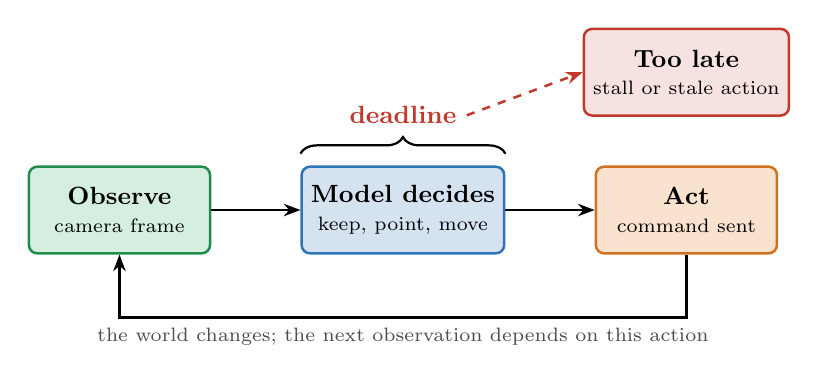
\begin{tikzpicture}[
  every node/.style={font=\small},
  box/.style={draw, rounded corners=3pt, minimum width=2.3cm, minimum height=1.1cm,
              align=center, line width=0.9pt},
  arr/.style={-{Stealth[length=6pt]}, line width=0.9pt},
  lbl/.style={font=\scriptsize, text=black!70}
]
  \node[box, fill=green2!20, draw=green2!80!black]   (obs) at (0,0)   {\textbf{Observe}\\[-1pt]{\scriptsize camera frame}};
  \node[box, fill=accent!20, draw=accent]            (dec) at (3.6,0) {\textbf{Model decides}\\[-1pt]{\scriptsize keep, point, move}};
  \node[box, fill=orange2!22, draw=orange2!90!black] (act) at (7.2,0) {\textbf{Act}\\[-1pt]{\scriptsize command sent}};
  \draw[arr] (obs) -- (dec);
  \draw[arr] (dec) -- (act);
  \draw[arr] (act.south) -- ++(0,-0.8) -| (obs.south)
    node[pos=0.25, below, lbl] {the world changes; the next observation depends on this action};

  \draw[decorate, decoration={brace, amplitude=6pt}, line width=0.8pt]
    ($(dec.north west)+(0,0.15)$) -- ($(dec.north east)+(0,0.15)$)
    node[midway, above=7pt, font=\small\bfseries, text=red2] (dl) {deadline};

  \node[box, fill=red2!14, draw=red2, minimum width=2.6cm] (miss) at (7.2,1.75)
    {\textbf{Too late}\\[-1pt]{\scriptsize stall or stale action}};
  \draw[arr, red2, dashed] (dl.east) -- (miss.west);
\end{tikzpicture}}
\end{center}
\vfill

\end{frame}

% ==================================================================
\begin{frame}{Looped use cases: two in space, two on robots.}

\vspace{0.1cm}
\small
We can make inference \textbf{faster}, but more importantly \textbf{more deterministic}.

\vspace{0.1cm}
\begin{center}
\footnotesize
\raggedright
\renewcommand{\arraystretch}{1.45}
\setlength{\tabcolsep}{4pt}
\setlength{\aboverulesep}{0pt}
\setlength{\belowrulesep}{0pt}
\begin{tabular}{>{\raggedright\arraybackslash}p{0.17\linewidth}|>{\raggedright\arraybackslash}p{0.21\linewidth}|>{\raggedright\arraybackslash}p{0.32\linewidth}|>{\raggedright\arraybackslash}p{0.09\linewidth}|>{\raggedright\arraybackslash}p{0.10\linewidth}}
\toprule
\textbf{Use case} & \textbf{Deadline} & \textbf{Evidence} & \textbf{Slow?} & \textbf{Jitter?} \\
\midrule
Image triage\newline{\scriptsize space, VLM} & Before the next image arrives (1--30\,s) & 26.6\,s per image on the ground vs.\ 20\,s between images \href{https://arxiv.org/abs/2606.18271}{\underline{paper}} & \textcolor{red2}{\textbf{yes}} & \textcolor{orange2}{\textbf{?}} \\
Retasking\newline{\scriptsize space, VLM} & Before the target leaves view & Kepler says it does this, no numbers yet & \textcolor{orange2}{\textbf{?}} & \textcolor{orange2}{\textbf{?}} \\
Fast manipulation\newline{\scriptsize robot, VLA} & About 50\,ms & Ping-pong hits: 0/20 sync vs.\ 11/20 async \href{https://arxiv.org/abs/2512.01031}{\underline{paper}} & \textcolor{red2}{\textbf{yes}} & \textcolor{orange2}{\textbf{?}} \\
Onboard control\newline{\scriptsize robot, VLA} & Before the current actions run out & Cloth folding: 0/10 on Orin vs.\ 7/10 on a 4090 \href{https://arxiv.org/abs/2607.12659}{\underline{paper}} & \textcolor{red2}{\textbf{yes}} & \textcolor{orange2}{\textbf{?}} \\
\bottomrule
\end{tabular}
\end{center}

\vspace{0.2cm}
\small
\textbf{Slow} is what prior work fixes. \textbf{?} means the papers report no jitter, so we do not know if the slow requests are rare or routine.

\end{frame}

% ==================================================================
\begin{frame}{Prior work: fast on average, or predictable for DNNs only.}

\vspace{0.4cm}
\begin{columns}[T,onlytextwidth]
\column{0.31\textwidth}
\begin{block}{Datacenter LLM serving}
  \small
  \textbf{Fast on average.}\\[0.3em]
  {\scriptsize\color{gray2} DistServe, Sarathi-Serve, SOLA}
\end{block}
\column{0.31\textwidth}
\begin{block}{Real-time GPU work}
  \small
  \textbf{Predictable, but only for DNNs.}\\[0.3em]
  {\scriptsize\color{gray2} Clockwork, REEF, TimeGraph}
\end{block}
\column{0.31\textwidth}
\begin{block}{Our setting}
  \small
  \textbf{An LLM in a loop on a Jetson.}\\[0.3em]
  {\scriptsize\color{gray2} One late answer breaks the loop}
\end{block}
\end{columns}

\vspace{0.9cm}
\begin{center}
\begin{minipage}{0.85\textwidth}
\begin{block}{The gap}
  \small
  Nobody measures how often an LLM misses its deadline in a loop on a Jetson.
\end{block}
\end{minipage}
\end{center}

\vfill
{\scriptsize\color{gray2} Full table with numbers: \hyperlink{priortable}{\underline{appendix}}.}

\end{frame}

% ==================================================================
\begin{frame}{Measurement setup: real device under test, simulated world.}

\vspace{0.25cm}
\begin{center}
\resizebox{\linewidth}{!}{%
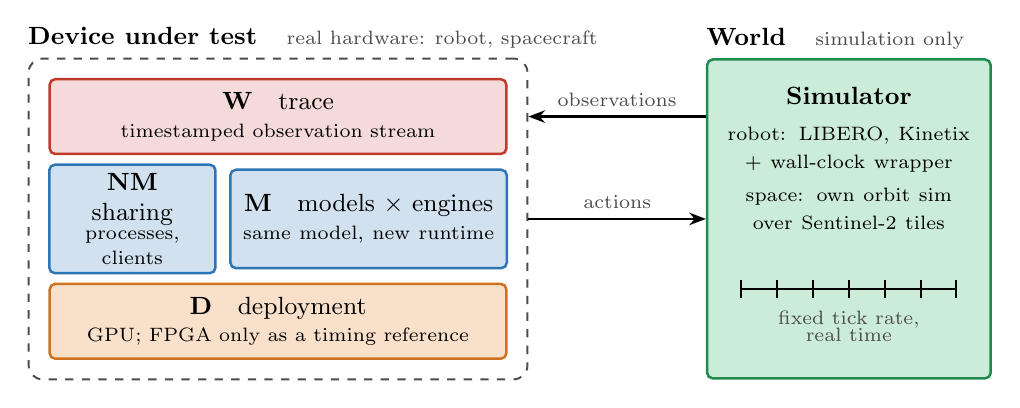
\begin{tikzpicture}[
  every node/.style={font=\small},
  blk/.style={draw, rounded corners=2pt, minimum height=0.95cm, align=center,
              line width=0.9pt, inner sep=3pt},
  arr/.style={-{Stealth[length=6pt]}, line width=0.9pt},
  lbl/.style={font=\scriptsize, text=black!70},
  head/.style={font=\small\bfseries, anchor=south west, inner sep=0pt, yshift=3pt}
]
  % ---- device under test ----
  \node[blk, minimum width=5.8cm, fill=red2!18, draw=red2] (W) at (0,2.6)
    {\textbf{W}\quad trace\\[-1pt]{\scriptsize timestamped observation stream}};
  \node[blk, text width=1.9cm, minimum height=1.25cm, fill=accent!22, draw=accent] (NM) at (-1.85,1.3)
    {\textbf{NM}\quad sharing\\[-1pt]{\scriptsize processes,\\[-2pt] clients}};
  \node[blk, text width=3.3cm, minimum height=1.25cm, fill=accent!22, draw=accent] (M) at (1.15,1.3)
    {\textbf{M}\quad models $\times$ engines\\[-1pt]{\scriptsize same model, new runtime}};
  \node[blk, minimum width=5.8cm, fill=orange2!24, draw=orange2!90!black] (D) at (0,0)
    {\textbf{D}\quad deployment\\[-1pt]{\scriptsize GPU; FPGA only as a timing reference}};
  \begin{scope}[on background layer]
    \node[draw=black!70, dashed, line width=0.7pt, rounded corners=5pt, fit=(W)(NM)(M)(D), inner sep=7pt] (DEV) {};
  \end{scope}
  \node[head] at (DEV.north west)
    {Device under test\quad{\mdseries\scriptsize\color{black!70} real hardware: robot, spacecraft}};

  % ---- world (same height as the device box) ----
  \node[blk, minimum width=3.6cm, minimum height=4.05cm, fill=green2!24, draw=green2!80!black]
    (ENV) at (7.25,1.3) {};
  \node[head] at (ENV.north west)
    {World\quad{\mdseries\scriptsize\color{black!70} simulation only}};
  \node[anchor=north, align=center, text width=3.5cm, inner xsep=0pt, yshift=-7pt] at (ENV.north) {%
      \textbf{Simulator}\\[5pt]
      {\scriptsize robot: LIBERO, Kinetix\\[-1pt] + wall-clock wrapper}\\[4pt]
      {\scriptsize space: own orbit sim\\[-1pt] over Sentinel-2 tiles}};
  % fixed-rate tick strip
  \coordinate (t0) at ($(ENV.south west)+(0.45,1.15)$);
  \coordinate (t1) at ($(ENV.south east)+(-0.45,1.15)$);
  \draw[line width=0.7pt] (t0) -- (t1);
  \foreach \i in {0,...,6} {
    \draw[line width=0.7pt] ($(t0)!\i/6!(t1)$) ++(0,-0.11) -- ++(0,0.22);
  }
  \node[lbl, anchor=north, align=center] at ($(t0)!0.5!(t1)+(0,-0.16)$) {fixed tick rate,\\[-2pt] real time};

  % ---- loop ----
  \draw[arr] (ENV.west |- W.east) -- (DEV.east |- W.east) node[midway, above, lbl] {observations};
  \draw[arr] (DEV.east |- M.east) -- (ENV.west |- M.east) node[midway, above, lbl] {actions};
\end{tikzpicture}}
\end{center}

\vspace{0.3cm}
\small
\begin{itemize}
  \setlength{\itemsep}{0.4em}
  \item \textbf{Real device, simulated world:} no real robot or orbit in this study.
  \item \textbf{Simulator:} takes actions, steps its world, emits observations.
  \item \textbf{The world never waits for M:} a miss hurts the task, as in reality.
\end{itemize}

\end{frame}
% ==================================================================
\begin{frame}{First experiment: a small LLM on a Jetson, fed at a fixed rate.}

\vspace{0.3cm}
\begin{center}
\resizebox{0.95\linewidth}{!}{%
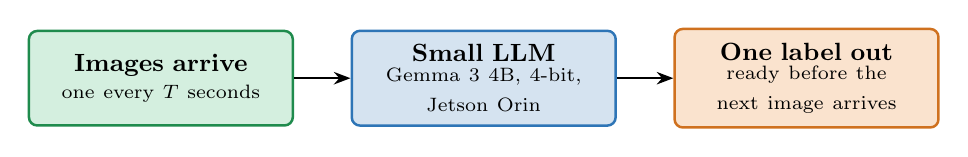
\begin{tikzpicture}[
  every node/.style={font=\small},
  box/.style={draw, rounded corners=3pt, text width=3.0cm, minimum height=1.2cm, align=center, line width=0.9pt, inner sep=5pt},
  arr/.style={-{Stealth[length=6pt]}, line width=0.9pt}
]
  \node[box, fill=green2!20, draw=green2!80!black]   (in)  at (0,0)   {\textbf{Images arrive}\\[-1pt]{\scriptsize one every $T$ seconds}};
  \node[box, fill=accent!20, draw=accent]            (llm) at (4.1,0) {\textbf{Small LLM}\\[-1pt]{\scriptsize Gemma 3 4B, 4-bit,\\ Jetson Orin}};
  \node[box, fill=orange2!22, draw=orange2!90!black] (out) at (8.2,0) {\textbf{One label out}\\[-1pt]{\scriptsize ready before the\\ next image arrives}};
  \draw[arr] (in) -- (llm);
  \draw[arr] (llm) -- (out);
\end{tikzpicture}}
\end{center}

\vspace{0.5cm}
\begin{columns}[T,onlytextwidth]
\column{0.31\textwidth}
\begin{block}{We vary}
  \small
  Model alone. Then with other processes. Then at a lower power mode.
\end{block}
\column{0.31\textwidth}
\begin{block}{We record}
  \small
  Latency of every single request, plus energy and clock speed.
\end{block}
\column{0.31\textwidth}
\begin{block}{We ask}
  \small
  How often is the label late, and which change makes it late?
\end{block}
\end{columns}

\end{frame}

% ==================================================================
\begin{frame}{What we want vs.\ what we get: the long tail is the miss.}

\begin{columns}[T,onlytextwidth]
\column{0.5\textwidth}
\begin{center}
{\small\bfseries\color{green2!70!black} What we want}\\[2pt]
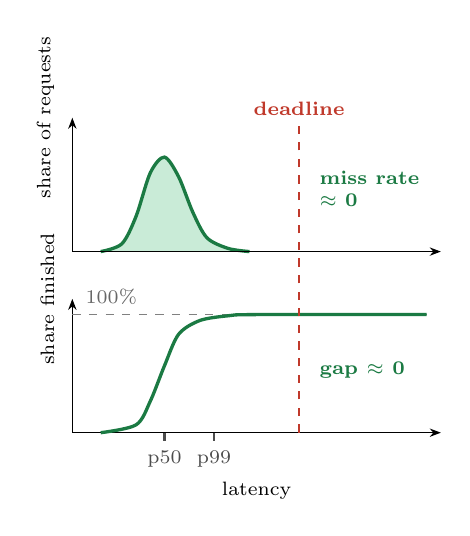
\begin{tikzpicture}[x=0.9cm, y=0.5cm, every node/.style={font=\scriptsize},
  axis/.style={black, line width=0.5pt, -{Stealth[length=4pt]}}]
  \fill[green2!25] plot[smooth] coordinates {(0.4,0) (0.7,0.2) (0.9,0.9) (1.1,2.0) (1.3,2.4) (1.5,1.9) (1.7,1.0) (1.9,0.35) (2.2,0.08) (2.5,0)} -- cycle;
  \draw[green2!70!black, line width=1.2pt] plot[smooth] coordinates {(0.4,0) (0.7,0.2) (0.9,0.9) (1.1,2.0) (1.3,2.4) (1.5,1.9) (1.7,1.0) (1.9,0.35) (2.2,0.08) (2.5,0)};
  \draw[axis] (0,0) -- (5.2,0);
  \draw[axis] (0,0) -- (0,3.4) node[left, rotate=90, anchor=south, yshift=3pt] {share of requests};
  \node[green2!70!black, anchor=west, align=left] at (3.35,1.6) {\textbf{miss rate}\\ \textbf{$\approx$ 0}};
  \begin{scope}[yshift=-2.3cm]
  \draw[axis] (0,0) -- (5.2,0);
  \draw[axis] (0,0) -- (0,3.4) node[left, rotate=90, anchor=south, yshift=3pt] {share finished};
  \node[anchor=south west, black!60] at (0.05,3.0) {100\%};
  \draw[dashed, black!50] (0,3.0) -- (5.0,3.0);
  \draw[green2!70!black, line width=1.2pt] plot[smooth] coordinates {(0.4,0) (0.9,0.2) (1.1,0.8) (1.3,1.7) (1.5,2.5) (1.8,2.85) (2.2,2.97) (2.6,3.0) (5.0,3.0)};
  \node[green2!70!black, anchor=west, align=left] at (3.35,1.6) {\textbf{gap $\approx$ 0}};
  \draw[black!70, line width=0.8pt] (1.3,0) -- (1.3,-0.2) node[below] {p50};
  \draw[black!70, line width=0.8pt] (2.0,0) -- (2.0,-0.2) node[below] {p99};
  \node[anchor=north] at (2.6,-1.0) {latency};
  \end{scope}
  \draw[red2, line width=1pt, dashed] (3.2,-4.6) -- (3.2,3.2) node[above] {\textbf{deadline}};
\end{tikzpicture}
\end{center}
\column{0.5\textwidth}
\begin{center}
{\small\bfseries\color{red2} What we get today}\\[2pt]
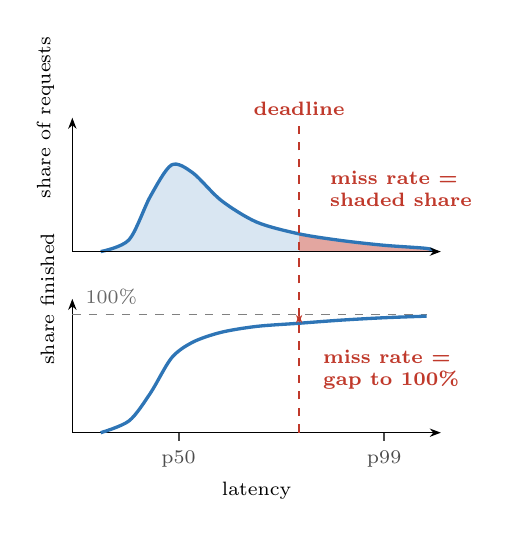
\begin{tikzpicture}[x=0.9cm, y=0.5cm, every node/.style={font=\scriptsize},
  axis/.style={black, line width=0.5pt, -{Stealth[length=4pt]}}]
  \fill[accent!18] plot[smooth] coordinates {(0.4,0) (0.8,0.3) (1.1,1.4) (1.4,2.2) (1.7,2.0) (2.1,1.3) (2.6,0.75) (3.2,0.45) (3.8,0.28) (4.4,0.16) (5.0,0.08) (5.1,0)} -- cycle;
  \begin{scope}
    \clip (3.2,0) rectangle (5.3,3.0);
    \fill[red2!45] plot[smooth] coordinates {(0.4,0) (0.8,0.3) (1.1,1.4) (1.4,2.2) (1.7,2.0) (2.1,1.3) (2.6,0.75) (3.2,0.45) (3.8,0.28) (4.4,0.16) (5.0,0.08) (5.1,0)} -- cycle;
  \end{scope}
  \draw[accent, line width=1.2pt] plot[smooth] coordinates {(0.4,0) (0.8,0.3) (1.1,1.4) (1.4,2.2) (1.7,2.0) (2.1,1.3) (2.6,0.75) (3.2,0.45) (3.8,0.28) (4.4,0.16) (5.0,0.08) (5.1,0)};
  \draw[axis] (0,0) -- (5.2,0);
  \draw[axis] (0,0) -- (0,3.4) node[left, rotate=90, anchor=south, yshift=3pt] {share of requests};
  \node[red2, anchor=south west, align=left] at (3.5,0.9) {\textbf{miss rate =}\\ \textbf{shaded share}};
  \begin{scope}[yshift=-2.3cm]
  \draw[axis] (0,0) -- (5.2,0);
  \draw[axis] (0,0) -- (0,3.4) node[left, rotate=90, anchor=south, yshift=3pt] {share finished};
  \node[anchor=south west, black!60] at (0.05,3.0) {100\%};
  \draw[dashed, black!50] (0,3.0) -- (5.0,3.0);
  \draw[accent, line width=1.2pt] plot[smooth] coordinates {(0.4,0) (0.8,0.3) (1.1,1.0) (1.4,1.9) (1.7,2.3) (2.1,2.55) (2.6,2.7) (3.2,2.78) (3.8,2.86) (4.4,2.92) (5.0,2.96)};
  \draw[{Stealth[length=3pt]}-{Stealth[length=3pt]}, red2, line width=0.9pt] (3.2,2.78) -- (3.2,3.0);
  \node[red2, anchor=west, align=left] at (3.4,1.6) {\textbf{miss rate =}\\ \textbf{gap to 100\%}};
  \draw[black!70, line width=0.8pt] (1.5,0) -- (1.5,-0.2) node[below] {p50};
  \draw[black!70, line width=0.8pt] (4.4,0) -- (4.4,-0.2) node[below] {p99};
  \node[anchor=north] at (2.6,-1.0) {latency};
  \end{scope}
  \draw[red2, line width=1pt, dashed] (3.2,-4.6) -- (3.2,3.2) node[above] {\textbf{deadline}};
\end{tikzpicture}
\end{center}
\end{columns}

\vspace{-0.1cm}
\scriptsize
\begin{itemize}
  \setlength{\itemsep}{0.2em}
  \item \textbf{Top:} share of requests at each latency. \textbf{Bottom:} share finished by then.
  \item \textbf{Miss rate:} the shaded tail on top, the gap to 100\% below.
\end{itemize}

\end{frame}

% ==================================================================
\begin{frame}{What we measure per request.}

\vspace{0.2cm}
\begin{center}
\small
\raggedright
\renewcommand{\arraystretch}{1.6}
\setlength{\aboverulesep}{0pt}
\setlength{\belowrulesep}{0pt}
\begin{tabular}{>{\raggedright\arraybackslash}p{0.30\linewidth}|>{\raggedright\arraybackslash}p{0.60\linewidth}}
\toprule
\textbf{Metric} & \textbf{In plain words} \\
\midrule
Time to first token & How long until the model starts answering. Split into waiting and prefill. \\
Time between tokens & How steadily the answer streams out. \\
Time to last token & Total time for the request. \\
Miss rate & Share of requests that finish after the deadline. \\
Tail ratio (p99 / p50) & How much worse the slow requests are than the typical one. \\
Energy per request & Joules, with clock speed, so throttling shows up. \\
\bottomrule
\end{tabular}
\end{center}

\vspace{0.3cm}
\small
With one-token answers, first token and last token are the same, so only prefill and the miss rate are left.

\end{frame}

% ==================================================================
\appendix

\begin{frame}[plain]
  \vfill
  \begin{center}
    {\Large\bfseries Appendix}\\[0.8em]
    \small Broader use cases, agentic framing, sources.
  \end{center}
  \vfill
\end{frame}

\begin{frame}{Latency-bound inference: use cases from well-known groups.}

\begin{center}
\footnotesize
\raggedright
\renewcommand{\arraystretch}{1.2}
\setlength{\aboverulesep}{0pt}
\setlength{\belowrulesep}{0pt}
\begin{tabular}{>{\raggedright\arraybackslash}p{0.17\linewidth}|>{\raggedright\arraybackslash}p{0.19\linewidth}|>{\raggedright\arraybackslash}p{0.40\linewidth}|>{\raggedright\arraybackslash}p{0.18\linewidth}}
\toprule
\textbf{Domain} & \textbf{Use case} & \textbf{Evidence} & \textbf{Setup} \\
\midrule
Space & Image filtering & Earth+: only 2\% of captured image data can be downloaded (citing Kodan) \href{https://arxiv.org/abs/2403.11434}{\underline{paper}} & Constellation \\
Space & VLM queries & Gemma 3 4B classifies live imagery onboard, April 2026 \href{https://arxiv.org/abs/2606.18271}{\underline{paper}} & Jetson Orin AGX \\
Physical AI & Robot manipulation & VLASH: reaction latency 546--565\,ms sync vs.\ 46--65\,ms async \href{https://arxiv.org/abs/2512.01031}{\underline{paper}} & RTX 5090, SO-101 \\
Physical AI & Onboard VLA control & Jetson-PI: 8.66$\times$ control rate over naive PyTorch \href{https://arxiv.org/abs/2607.12659}{\underline{paper}} & Jetson Orin \\
Physics & Level-1 trigger & hls4ml jet tagger: about 100\,ns (2018) \href{https://arxiv.org/abs/1804.06913}{\underline{paper}} & FPGA \\
\bottomrule
\end{tabular}
\end{center}

\end{frame}



\begin{frame}[shrink=8]{Agentic use cases: the orbit sets the deadline, not the token rate.}

\begin{center}
\scriptsize
\raggedright
\renewcommand{\arraystretch}{1.15}
\setlength{\tabcolsep}{3pt}
\setlength{\aboverulesep}{0pt}
\setlength{\belowrulesep}{0pt}
\begin{tabular}{>{\raggedright\arraybackslash}p{0.15\linewidth}|>{\raggedright\arraybackslash}p{0.24\linewidth}|>{\raggedright\arraybackslash}p{0.21\linewidth}|>{\raggedright\arraybackslash}p{0.33\linewidth}}
\toprule
\textbf{Use case} & \textbf{Agent decision} & \textbf{Deadline (source)} & \textbf{Evidence} \\
\midrule
Capture triage & Label, keep or drop, one-line description per frame & Inter-capture cadence: 1--30\,s (Kodan), 20\,s claimed in flight & NAVI-Orbital: Gemma 3 4B, 4-bit, Orin AGX; 26.6\,s ground cycle vs.\ 20\,s cadence; retries unbounded \href{https://arxiv.org/abs/2606.18271}{\underline{paper}} \\
Closed-loop retasking & Slew or zoom for the next capture after a wide-FOV detection & Remaining access window: seconds to minutes & Kepler retasking claim (operator, no numbers); the one case where a late decision changes the next observation \\
Pre-contact packaging & Rank and summarize what to downlink & Contact start, known ahead from SGP4 & Earth+: 2\% of image data can come down \href{https://arxiv.org/abs/2403.11434}{\underline{paper}}; wildfire alerts delayed up to 90\,min \href{https://spectrum.ieee.org/nasa-ai-satellite-image-analysis}{\underline{news}} \\
In-pass operator query & Answer an uplinked question over the onboard log & Same contact window (minutes), else next pass & NAVI dialogue agent; output length varies, so tokens trade directly against the deadline \\
\bottomrule
\end{tabular}
\end{center}

\vspace{0.15cm}
\footnotesize
\begin{itemize}
  \setlength{\itemsep}{0.25em}
  \item \textbf{Metric:} deadline-miss rate at a fixed budget, plus task quality at that budget. No paper in the review reports a miss rate.
  \item \textbf{Single-token output:} fixed image tokens plus one label is fixed-shape prefill, the regime Jetson-PI's CUDA-graph reuse exploits.
\end{itemize}

\end{frame}

\begin{frame}{Agentic physical AI candidates from the lit review.}

\begin{center}
\footnotesize
\raggedright
\renewcommand{\arraystretch}{1.2}
\setlength{\aboverulesep}{0pt}
\setlength{\belowrulesep}{0pt}
\begin{tabular}{>{\raggedright\arraybackslash}p{0.22\linewidth}|>{\raggedright\arraybackslash}p{0.40\linewidth}|>{\raggedright\arraybackslash}p{0.30\linewidth}}
\toprule
\textbf{Use case} & \textbf{Why it is agentic} & \textbf{Latency evidence} \\
\midrule
Navigation among people & Reasoning step picks the route while people move & TIC-VLA / DynaNav: reasoning delay injected \href{https://arxiv.org/abs/2602.02459}{\underline{paper}} \\
Split planner and policy & Large model on a workstation plans, small model on the robot acts & AsyncVLA: enforced latency up to 6\,s \href{https://arxiv.org/abs/2602.13476}{\underline{paper}} \\
Subtask sequencing & Pick, fold, place could sit under a planner & Jetson-PI uses one VLA for all three \href{https://arxiv.org/abs/2607.12659}{\underline{paper}} \\
\bottomrule
\end{tabular}
\end{center}

\vspace{0.3em}
\small
All delays here are injected or enforced. None is a measured deadline-miss rate.

\end{frame}

\begin{frame}[label=priortable]{Prior work on meeting deadlines: what exists, and what is missing.}

\begin{center}
\scriptsize
\raggedright
\renewcommand{\arraystretch}{1.45}
\setlength{\aboverulesep}{0pt}
\setlength{\belowrulesep}{0pt}
\begin{tabular}{>{\raggedright\arraybackslash}p{0.22\linewidth}|>{\raggedright\arraybackslash}p{0.17\linewidth}|>{\raggedright\arraybackslash}p{0.29\linewidth}|>{\raggedright\arraybackslash}p{0.22\linewidth}}
\toprule
\textbf{Work} & \textbf{Setting} & \textbf{What it shows} & \textbf{What is missing} \\
\midrule
DistServe, OSDI '24 \href{https://www.usenix.org/conference/osdi24/presentation/zhong-yinmin}{\underline{paper}} & Datacenter LLM serving & Splitting prefill and decode serves 7.4$\times$ more requests within the SLO & Targets 90\% of requests, not all \\
Sarathi-Serve, OSDI '24, Microsoft \href{https://www.usenix.org/conference/osdi24/presentation/agrawal}{\underline{paper}} & Datacenter LLM serving & Chunked prefill stops new requests stalling running ones & Throughput goal, no deadline \\
SOLA, MLSys '25 \href{https://mlsys.org/virtual/2025/3345}{\underline{paper}} & Datacenter LLM serving & SLO attainment from 45.5\% to 99.4\% & Best effort, no guarantee \\
Clockwork, OSDI '20 \href{https://www.usenix.org/conference/osdi20/presentation/gujarati}{\underline{paper}} & DNN serving & 100\,ms met for 99.997\% of requests & Fixed-size DNNs, no decode \\
TimeGraph, ATC '11, CMU \href{https://www.usenix.org/conference/usenixatc11/timegraph-gpu-scheduling-real-time-multi-tasking-environments}{\underline{paper}} & Real-time GPU scheduling & Priorities and reservations protect key GPU tasks & Graphics era, not ML \\
REEF, OSDI '22 \href{https://www.usenix.org/conference/osdi22/presentation/han}{\underline{paper}} & Real-time DNN serving & Preempts GPU kernels in microseconds & DNNs, datacenter GPU \\
\bottomrule
\end{tabular}
\end{center}

\vspace{0.2em}
\small
\textbf{Gap:} LLM serving targets averages in datacenters. Real-time GPU work stops at DNNs. Nobody measures LLM misses in a loop on a Jetson.

\end{frame}

% ==================================================================
% BACKUP: the old right-hand plot, moved out of the main flow
\begin{frame}{What deadline can the device promise?}

\vspace{0.2cm}
\begin{center}
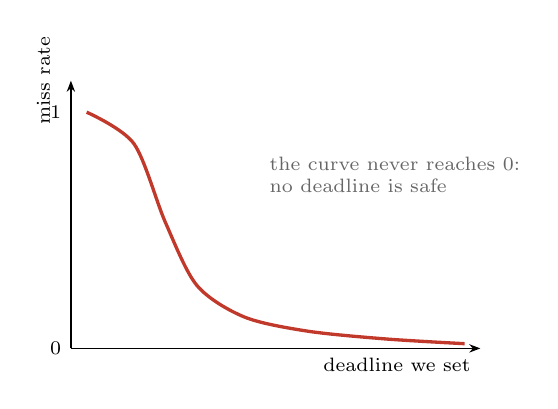
\begin{tikzpicture}[scale=1.0, every node/.style={font=\scriptsize},
  axis/.style={black, line width=0.5pt, -{Stealth[length=4pt]}}]
  \draw[axis] (0,0) -- (5.2,0) node[below left] {deadline we set};
  \draw[axis] (0,0) -- (0,3.4) node[left, rotate=90, anchor=south, yshift=4pt] {miss rate};
  \node[left] at (0,3.0) {1};
  \node[left] at (0,0) {0};
  \draw[red2, line width=1.2pt] plot[smooth] coordinates
    {(0.2,3.0) (0.8,2.6) (1.2,1.6) (1.6,0.8) (2.2,0.4) (3.0,0.22) (4.0,0.12) (5.0,0.06)};
  \node[black!60, anchor=west, align=left] at (2.4,2.2) {the curve never reaches 0:\\ no deadline is safe};
\end{tikzpicture}
\end{center}

\small
Each point is the miss rate at one deadline. Read it right to left: a longer deadline lowers the miss rate, but a long tail keeps it above zero.

\end{frame}

\begin{frame}[shrink=10]{Sources}

\footnotesize
\begin{itemize}
  \setlength{\itemsep}{0.25em}
  \item \href{https://arxiv.org/abs/2403.11434}{Earth+ (ASPLOS 2025)}
  \item \href{https://arxiv.org/abs/2606.18271}{NAVI-Orbital: Gemma 3 on Loft YAM-9 (arXiv 2606.18271)}
  \item \href{https://spectrum.ieee.org/nasa-ai-satellite-image-analysis}{Loft YAM-9 coverage (news, IEEE Spectrum)}
  \item \href{https://arxiv.org/abs/2512.01031}{VLASH, asynchronous VLA inference (arXiv 2512.01031)}
  \item \href{https://arxiv.org/abs/2607.12659}{Jetson-PI, onboard VLA control (CoRL 2026)}
  \item \href{https://arxiv.org/abs/1804.06913}{hls4ml, fast DNN inference in FPGAs (arXiv 1804.06913)}
  \item \href{https://arxiv.org/abs/2602.02459}{TIC-VLA / DynaNav (arXiv 2602.02459, ICML 2026)}
  \item \href{https://arxiv.org/abs/2602.13476}{AsyncVLA (Levine group, UC Berkeley; arXiv 2602.13476)}
  \item \href{https://www.usenix.org/conference/osdi24/presentation/zhong-yinmin}{DistServe (OSDI 2024)}
  \item \href{https://www.usenix.org/conference/osdi24/presentation/agrawal}{Sarathi-Serve (OSDI 2024, Microsoft Research)}
  \item \href{https://mlsys.org/virtual/2025/3345}{SOLA (MLSys 2025)}
  \item \href{https://www.usenix.org/conference/osdi20/presentation/gujarati}{Clockwork (OSDI 2020)}
  \item \href{https://www.usenix.org/conference/usenixatc11/timegraph-gpu-scheduling-real-time-multi-tasking-environments}{TimeGraph (USENIX ATC 2011)}; \href{https://www.usenix.org/conference/osdi22/presentation/han}{REEF (OSDI 2022)}
\end{itemize}

\end{frame}

\end{document}
